\documentclass[12pt, 
    twoside=false, 
    bibliography=totoc, 
    numbers=endperiod, 
    headings=normal, 
    toc=chapterentrydotfill
    ]{scrbook}
\usepackage[T1]{fontenc}
\usepackage[utf8]{inputenc}
\usepackage[ngerman]{babel}
\usepackage{blindtext}
\usepackage{csquotes}
\usepackage{booktabs}
\usepackage{setspace}
\usepackage{mathpazo}
\usepackage{graphicx}
\usepackage{etoolbox}
\usepackage[
  	pdfstartview=FitH,   
  	pdffitwindow=true,
  	colorlinks,
  	linkcolor=black,
  	anchorcolor=black,
  	citecolor=black,
  	urlcolor=black
  	]{hyperref}
\usepackage[labelfont=bf]{caption}
\usepackage{float}
\usepackage[
    backend=biber, 
    style=authoryear-ibid, 
    eprint=false,
    url=false,
    doi=false,
    isbn=false,
    dashed=false
    ]{biblatex}
\addbibresource{Bib.bib}

% Layoutanpassungen
\setkomafont{sectioning}{\normalcolor\bfseries}
\renewcommand*{\chapterheadstartvskip}{\vspace*{-\topskip}}
\KOMAoptions{headsepline = true}
\setlength{\textheight}{1.05\textheight}
\AtBeginEnvironment{quote}{\singlespacing\small}

\begin{document}

\begin{titlepage}
    \begin{minipage}[t]{0.6\textwidth}
    \flushleft 
    Universität Hamburg \\
    Fachbereich: Sozialwissenschaften \\
    Fachgebiet: Politikwissenschaft \\
    Seminar: Forschungsseminar Vergleichende und Regionalstudien \\ 
    Dozenten: Prof. Kai-Uwe Schnapp \\
    PD Dr. Falk Daviter \\
    Wintersemester 2018/19 \\
    \end{minipage}
    \hfill
    \begin{minipage}[t][1.7cm][b]{0.35\textwidth}
    
\includegraphics[width=\textwidth]{images/UHH-Logo_2010_Farbe_CMYK.pdf}
    \end{minipage}
    
    \vspace*{\fill}
    \begin{center}
	\vspace{1cm}\noindent {\textbf{Projektarbeit}} \vspace{0.2cm} \\
	\textbf{\Large Geschlechtsbezogene Partizipationsunterschiedein Parlamentsdebatten  oder Geschlechtsbezogene Repräsentationsunterschiede in Parlamentsdebatten (ich finde zweites sinnvoller) \\
	\vspace {0,5cm} \small\emph{Inwieweit unterscheiden sich Redebeiträge und Verhalten von weiblichen und männlichen Abgeordneten im 19. Deutschen Bundestag bezüglich Häufigkeit, Thematik und Geschlechterneutralität}} \\
	\vspace{0.5cm}
	30.03.2019
	\end{center}
    \vspace*{\fill}
	
	\begin{minipage}[t]{0.48\textwidth}
    \flushleft 
    Gina-Gabriela Görner \\
    Matrikelnummer: 6436971 \\
    XXX \vspace{0.1cm} \\ 
	XXX \vspace{0.1cm}  \\
	E-Mail: Gina-Gabriela.Goerner@Studium.Uni-Hamburg.de \\ 
    \end{minipage}
    \begin{minipage}[t]{0.48\textwidth}
	\flushleft
	Josef Holnburger \\
	Matrikelnummer: XXX \\
	XXX \vspace{0.1cm} \\
	XXX \vspace{0.1cm} \\
	E-Mail: josef@holnburger.com \\
    \end{minipage}

\end{titlepage}

\frontmatter

\tableofcontents

\listoffigures
\addcontentsline{toc}{chapter}{\listfigurename}
\vspace*{24pt}
{\let\clearpage\relax \listoftables}	
\addcontentsline{toc}{chapter}{\listtablename}

\mainmatter

\setstretch{1.5}


\chapter{Einleitung}\label{Einleitung} 

\begin{quote}
     
 \enquote{Gender equal representation is not only about the proportion of men and women legislators or the
outcomes of politics}\parencite[197]{erikson_2018}
 \end{quote}

am Ende schreiben... 



Derzeit sind weniger als ein Viertel (24,3 %) Frauen in den weltweiten Parlamenten vertreten (http://archive.ipu.org/wmn-e/world.htm)


In demokratischen Systemen sind Parlamentarier nicht nur wichtige Akteure als GesetzgeberInnen, sondern auch als TeilnehmerInnen an der öffentlichen Debatte und als Mitwirkende an der öffentlichen Meinungsbildung  \parencite[188]{Dahlerup(closedcase)falls anderer gleiches jahr _2018}(ZOT aktualisieren!!!!). 

\begin{quote}
    
\enquote{
Gender equality in political representation may be described within both optimistic
and pessimistic stories.} \parencite[149]{celis und lovenduski _2018 schon in ZOT1}
\end{quote}

Repräsentative Institutionen werden trotz eines langen Kampfes um Gleichstellung noch immer von Männern dominiert (Celis und lov 2018,:: mit Verweis auf Childs und Lovenduski 2013:497-8, Dahlerup und Leyenaar 2013, Bjarnegard 2015 - alle schon in Zot aber noch nicht geprüft...). Frauen nehmen weniger als ein Viertel aller gesetzgebenden Sitze auf der ganzen Welt ein (Celis und lov 2018).Es ist nicht umstritten zu behaupten, dass die Gleichstellung der Geschlechter nicht erreicht wurde (Celis u lov 2018: 150) 

Die machtpolitische Gleichstellung der Geschlechter und politische Ressourcenverteilung in den industrialisierten Demokratien ist in den letzten fünfzig Jahren enorm gewachsen. (Coffe 2010: 318 - schon zot - noch laden). Es gibt mehr weibliche MPs als je zuvor und eine Rekordzahl von Frauen nimmt Führungspositionen in den Nationalen Regierungen (Lovenduski 2005; Paxton et .al 2007 noch nicht gecheckt, nicht zot) mit vielen wichtigen Konsequenzen für politische Ergebnisse und Prioritäten (Bolzendahl und Brooks 2007; Carroll 2001, Waring et al. - noch nicht gecheckt, nicht zot) ein (Coffe 2010: 318, schon zot - noch laden,) 


Repräsentation ist ein Kernkonzept in der Erforschung und Praxis der Politik und kann in drei verschiedene, miteinander verbundenen Dimensionen betrachtet werden. Es kann hierbei zwischen dem unterschieden werden, was repräsentiert wird, wie es repräsentiert wird und wer repräsentiert (Galligan 2007 :557). In den meisten Fällen bieten sowohl die WählerInnen, Parteien, Wahlen und GesetzgeberInnen den Hintergrund für eine Diskussion über eine oder mehrere Elemente der Repräsentation (Galligan 2007: 557, schon in zot - bitte laden) 
In der vorliegenden Arbeit….. 


Wichtig zu Beginn: Ziel der vorligeneden Arbeit ist die Untersuchunge der folgenden 5 Ebenen - welche jeweils in einem differezierten Verhältnis zum Repräsentationsbegriff stehen: 
\begin{itemize}
    \item Ebene 1: Repräsentation allgemein im Parlament : Anwesend/Abwesend/ Wie viele Frauen sind anwesend? 
    \item Ebene 2: Repräsentation allgemein in der Debatte: Teilnahme/Keine Teilnahme /Wie viel Teilnahme? 
    \item Ebene 3: Repräsentation Stereotypisierungen in der Debatte: unterschiedliche Themen/ gleiche Themen / Stereotypsierungen erfüllt/ nicht erfüllt ? 
    \item Ebene 4: Repräsentation innerhalb der Debatte: Einbeziehung von Frauen ja/nein in Form von: GFL ja/nein 
    \item Ebene 5: Repräsentation gesellschaftlichen Verhaltensmustern auch im Parlament - mehr Unterbrechungen / negative Unterbrechungen bei Frauen  ja/nein 
\end{itemize}

Wichtig zu betonen: Die Ebenen können nicht gänzlich voneinander unabhängig untersucht/ betrachtet werden, dennoch ist es notwenidg sie für eine komplexitätsreduktion vorerst zu differenzieren und in der Diskussion am Ende wieder zusammenzuführen .... 



\chapter{Theoretischer Hintergrund}

\section{Politik als Arbeitsperspektive} 
Dieses Kapitel muss noch überarbeitet werden!! 
Politics as a workplace ? (Kap orientiert an Erikson und Josefsson 2018) (alle genannte Lit ist bereits bei Zotero eingetragen - jedoch bisher noch nicht geprüft)  

Die bisherige Forschung zur politischen Repräsentation von Frauen fokussiert primär deskriptiven Themen, wie etwa die Frage danach, wie gesetzgebende Gremien durch Quoten geschlechtergerechter werden können  (vgl. Dahlerup and Freidenvall, 2005; Schwindt-Bayer, 2009 NOCH NICHT LIT geprüft aber Zotero hinzugefügt) oder  substantive Themen, welche beispielsweise untersuchen, ob weibliche Gesetzgeberinnen einen positiven Einfluss auf genderfreundliche politische Ergebnisse haben (Vgl. Beckwith and Cowell-Meyers, 2007 LIT noch prüfen, schon hinzugefügt Zotero) [ alles in Erikson, Josefsson 2018:199] \parencite[199]{erikson_2018}.

In Anlehnung an Erikson & Josefsson (2018) wurden den inneren Mechanismen der gesetzgebenden Körperschaften sowie der Frage, „how the political game itself is gendered“‘ (ebd.) weniger empirische Aufmerksamkeit gewidmet (siehe hierzu Childs, 2016; Dahlerup and Leyenaar, 2013; Wangnerud, 2015) (NOCH NICHT LIT geprüft aber Zotero hinzugefügt) [ alles in Erikson, Josefsson 2018:199] \parencite[199]{erikson_2018}.

Ein Ausgangspunkt der vorliegenden Arbeit ist, dass das legislative Arbeitsumfelds für sich genommen ebenso wichtig ist, wie die Möglichkeiten der weiblichen Gesetzgeberinnen, die Ergebnisse zu beeinflussen. Politikerinnen sollten in der Lage sein, ihre Aufgaben als Gesetzgeberinnen auf Augenhöhe mit ihren männlichen Kollegen erfüllen (Vgl. Erikson, Josefsson 2018:199) \parencite[199]{erikson_2018}. 

Dahlerup (1988, 2006 - Literatur noch nicht geprüft aber bei Zotero eingefügt)HIER WICHTIG; DAHLERUP LESEN ALS PRIMÄR) unterscheidet zwischen zwei verschiedenen Perspektiven der substantiellen Repräsentation von Frauen. Zum einen existiert die politische Outcome-Perspektive, welche die wissenschaftliche Literatur zur substantiellen Repräsentation von Frauen tendenziell dominiert. Zum anderen existiert die Perspektive der Politik als Arbeitsperspektive, welche bisher weniger häufig diskutiert wurde (Dahlerup 2006:513, SIEHE IN Erikson und Josefsson 2018: 199) \parencite[199]{erikson_2018}. 

Während sich die Outcome-Perspektive darauf konzentriert, ob weibliche Gesetzgeberinnen den Inhalt politischer Entscheidungen beeinflussen, indem sie diese geschlechterfreundlicher gestalten oder eine feministische Agenda verfolgen, beschäftigt sich die zweite Perspektive mit den Möglichkeiten, wie weibliche MPs als Repräsentantinnen gleichberechtigt mit ihren männlichen Kollegen auftreten können (Dahlerup 1988, 2006 Literatur noch nicht geprüft aber bei Zotero eingefügt - SIEHE In Erikson und Josefsson 2018: 199) \parencite[199]{erikson_2018}.

Der ‚workplace approach‘ (in Orientierung an Erikson und Josefsson 2018:199) zielt insgesamt darauf ab, die Repräsentation von Frauen aus einer breiteren Perspektive zu betrachten, indem der Fokus von den Ergebnissen auf die geschlechterspezifischen Bedingungen innerhalb der Legislative verlagert wird. In Anlehnung an Dahlerup (1988, 2006) und Erikson und Josefsson (2018:199) (WICHITG DAHLERUP LESEN!PRIMÄR), werden die Arbeitsbedingungen im deutschen Bundestag als wichtig eingestuft und als wesentlichen Bestandteil für die Möglichkeiten, wie Frauen die politischen Ergebnisse beeinflussen können, eingestuft  (Erikson und Josefsson 2018:199) \parencite[199]{erikson_2018}. noch sauber umschreiben!!!!

\section{Legislative Gremien als maskuline Organisation }


Orientiert an Erikson, Josefsson 2018:200 : Legislative bodies: Masculine and male-dominated organizations

-in Arbeit-

Innerhalb der legislativen Gremien wurde das Geschlechterregime ebenso wie in anderen von Männern dominierten Sektoren häufig als ‚permeated by a culture of masculinity‘ beschrieben (Lovenduski, 2005:  lit nicht geprüft aber in Zotero 48 und siehe in Erikson, Josefsson 2018:200)\parencite[200]{erikson_2018}. In Anlehnung an Acker 1990 zeigt sich dies beispielsweise in der Existenz von formalen Regeln, die von Männern geschaffen wurden und einer männlich dominierten Organisation angepasst sind. Außerdem in Normen, wie sich ein (männlicher) Politiker präsentieren und verhalten soll (vgl. Acker 1990 :  lit nicht geprüft aber in Zotero 48 und siehe in Erikson, Josefsson 2018:200) \parencite[200]{erikson_2018}. Frauen werden infolgedessen mit dieser bereits existierenden ‚culture of masculinity‘ konfrontiert, die als institutionelle Einschränkung fungieren kann, wenn ihre Arbeit dadurch behindert wird (Lovenduski 2005:47-56 nicht geprüft aber in Zotero 48 und siehe in Erikson, Josefsson 2018:200). Erikson und Josefsson 2018:200) \parencite[200]{erikson_2018} verweisen auf sozialpsychologische Forschungen, wonach Frauen in männerdominierten Bereichen häufig diskriminiert werden weil es an Übereinstimmungen zwischen den männerdominierten beruflichen Normen und den Eigenschaften mit denen Frauen typischerweise assoziiert werden mangelt (siehe hierzu Burgess und Borgida 1999; Eagly und Karau 2002; Heilmann 2001; Heilmann et al. 2004 --- schon in Zot aber noch nicht geprüft !!!))). Frauen riskieren demnach Diskriminierungen, weil sie entweder als weniger kompetent angesehen werden oder weil sie weibliche Attribute verletzen, wenn sie sich den Normen anpassen, so Erikson und Josefsson (2018:200) \parencite[200]{erikson_2018}. Die Folge sind neben der Disqualifikation die Abwertung der Leistungen von Frauen sowie die ungleiche Behandlung von Frauen, einschließlich von Belästigungen (Erikson und Josefsson 2018:200, \parencite[200]{erikson_2018}  siehe auch Burgess und Borgida 1999, Heilman 2001 – nicht geprüft, schon in zot)

\begin{quote}
     \endquote{The gendered consequences of masculine norms are often manifested in the first case in the disqualification of women or the devaluation of their performance, whereas they often take the form of a disparate treatment of women in the second, including harassment}\parencite[200]{erikson_2018}
\end{quote}

Informelle Praktiken und Normen können demnach als Hindernisse für die Schaffung eines geschlechtergerechten Arbeitsumfeldes angesehen werden \parencite[200]{erikson_2018}. 



\chapter{Relevanz des Forschungsgegenstandes}

\begin{itemize}
\item - Gleichberechtigung
\item -  Frauen im Parlament – zunehmend in der öffentlichen Debatte … 
\item -  die Zahl der Frauen im Parlament zunehmend in den Vordergrund der wissenschaftlichen Auseinandersetzung und der Politik. 
\end{itemize}

\begin{quote}
    \enquote{While women have made substantive progress in their representation in politics, they are still well underrepresented in political life in most nations} \parencite[2]{coffe_2013}
\end{quote}

Wenngleich ein politischer Konsens darin besteht, dass Gleichheit - und impliziert Geschlechtergleichheit- eine fundamentale Komponente von Demokratie darstellt, gibt es noch immer einen Gender-Gap in weltweit jedem Parlament (NOCH MAL PRÜFEN - ob Ruanda).  .... Repräsentation von Frauen für Demokratie notwendig .... 
…
\begin{itemize}
\item Anne Phillips gilt als eine der wichtigsten Vertreterinnen auf dem Gebiet der parlamentarischen Repräsentativität von Frauen. In ihrem Werk \emph{politics of presence} \parencite*{phillips_1998} analyisiert Phillips unter anderem die Bereitschaft von Frauen, als Parlamentskandidatin ausgewählt zu werden, Ministerin zu werden und Wahlen zu gewinnen \parencite[vgl.][416f.]{blaxill_2016}. 
Weil Frauen im täglichen Leben andere Erfahrungen sammeln als Männer -- insbesondere bezüglich der Kindererziehung, Bildung sowie der Auswahl an Berufen und der Unterscheidung von bezahlter und unbezahlter Arbeit, Gewalterfahrungen und sexuellen Belästigungen -- plädiert Philips für die notwendige Repräsentation von Frauen im Parlament, um andere Frauen vertreten zu können \parencite[vgl.][52]{wangnerud_2009}.
\end{itemize}

\begin{quote}
    \enquote{There are particular needs, interests, and concerns that arise from women's experience, and these will be inadequately addressed in a politics that is dominated by men. Equal rights to a vote have not proved strong enough to deal with this problem; there must also be equality among those elected to once} \parencite[66]{phillips_1998}
\end{quote}

Bereits Piktin \parencite*{pitkin_1972} argumentierte in ihrem Hauptwerk "The Concept of Representation", dass der Interessenbegriff in der Repräsentationsdebatte omnipräsent ("ubiquitious") ist \parencite[69]{wangnerud_2000}. Für Pitkin sind es die Parlamentarierinnen, welche sich den Wünschen und Interessen, dem Wohlergehen sowie Themen der Frauen widmen und diese vertreten \parencites[vgl.][413]{blaxill_2016}{pitkin_1972}. 

In Anlehnung an Phillips Theorie der \emph{politics of presence} \parencite*{phillips_1998} wird angenommen, dass weibliche Politikerinnen die Interessen und Wünsche weiblicher Bürgerinnen besser als männliche Politiker repräsentieren können. Hierbei wird die deskriptive mit der substantiellen Repräsentation verknüpft \parencite[52]{wangnerud_2009} : ein höherer Frauenanteil in Parlamenten führt zu einer stärkeren Thematisierung der Belange von Frauen.

\begin{itemize}
\item (Relevanz von Sprache: ) als Orientierung - nicht als Überschrift gedacht
\end{itemize}

Während die Forderungen einer deskriptiven parlamentarischen Geschlechtergleichheit bereits ihren Weg in die wissenschaftliche Diskussion und in die Politik gefunden haben, wurde der geschlechtergerechten Sprache sowie dem geschlechterbezogenen Verhalten in den Parlamenten bisher weniger Aufmerksamkeit gewidmet. 
Laut \textcite{menegatti_2017} ist die Sprache eine der einflussreichsten Faktoren, wodurch Sexismus und Geschlechterdiskriminierung gefördert und reproduziert werden \parencite*[1]{menegatti_2017}. Sprache kann hierbei insbesondere die sozialen Asymmetrien von Status und Macht zugunsten des Mannes reproduzieren (ebd.). Es existier[t]en einvernehmliche Normen, wonach der prototypische Mensch ein Mann ist, was sich in den Strukturen vieler Sprachen widerspiegelt und darin verankert ist. Viele grammatikalische und syntaktische Regeln sind so aufgebaut, dass weibliche Ausdrücke normalerweise von entsprechenden männlichen Formen abgeleitet werden (ebd.). Männliche Substantive und Pronomen werden beispielsweise häufig mit einer generischen Funktion verwendet um sich sowohl auf Männer als auch auf Frauen zu beziehen. Auf diese Weise verschwinden Frauen allerdings aus der mentalen Repräsentationen \parencites{vaughan_2018}{stahlberg_2001}. Maskuline Generika lassen Leser*innen und Hörer*innen mehr in männlichen als weiblichen Personenkategorien denken \parencites[2]{sczesny_2016}{stahlberg_2007}.

\begin{quote}
    \enquote{Given that language not only reflects stereotypical beliefs but also affects recipients’ cognition and behavior, the use of expressions consistent with gender stereotypes contributes to transmit and reinforce such belief system and can produce actual discrimination against women} \parencite[2]{menegatti_2017}
\end{quote}

\begin{itemize}
\item - CRITICAL MASS???  hier ggf noch 
\item - gendered -shelley et al ? (ich konnte dem Text nicht sehr viel entnehmen!) 
\item - Fehlt hier noch - Stereotypen als Theoretischer Unterbau und Unterbrechungen ...
\end{itemize}



\section {Derzeitiger Forschungsstand und relevante Studien }

\subsection{Frauen im Parlament}

In der Forschung zu Frauen im Parlament wird generell zwischen einer deskriptiven und einer substantiellen Repräsentation (in einigen Fällen zudem die symbolische Form der Repräsentation) unterschieden. Bei der substantiellen Repräsentation von Frauen handelt es sich um ein bisher weniger wissenschaftlich erforschtes Feld als die Analyse der deskriptiven Repräsentation \parencite[59]{wangnerud_2009}. 
Letzteres legt den Schwerpunkt auf die Analyse der Anzahl von Frauen in repräsentativen Institutionen, ersteres untersucht hingegen die Auswirkung der Präsenz von Frauen in Parlamenten \parencites[14]{coffe_2013}[52]{wangnerud_2009}.
Die zentralen Fragen lauten hierbei:

\begin{quote}
  \enquote{[W]hether the widely professed aspiration to feminise democracy -- and in so doing to politically empower women -- is a matter largely of symbolism or substance […]}
  \enquote{[…] wheter the priority should simply be to increase the proportion of women MPs in Parliament […] or as Hanna Pitkin argued in 1967, to represent minds as well as bodies.}
  \parencite[413]{blaxill_2016}
\end{quote}

%
Die zu Beginn erläuterte Theorie der \emph{politics of presence} \parencite{phillips_1998} diente Wängnerud \parencite*{wangnerud_2000} als Ausgangspunkt für ihre Forschung im Schwedischen Parlament (\enquote{Testing the Politics of Presence, Women's Representation in the Swedish Riksdag}, 2000). Wägnerud prüft hierbei die Hypothese, ob weibliche Politikerinnen die Interessen von Frauen stärker vertreten als männliche Politiker \parencite[84]{wangnerud_2000} und kommt zu folgendem Ergebnis: \enquote{[It is] difficult to repudiate the conclusion that women's interes are primarily represented by female politicians} \parencite[][84]{wangnerud_2000}. Laut Wängnerud \parencite*{wangnerud_2000} gibt es allerdings keine eindeutige Einschätzung darüber, welche Auswirkungen zu erwarten sind, wenn die Zahl der Frauen im Parlament steigt \parencite{wangnerud_2009}.
Die Forschung von \textcite{celis_2008} greift diese Annahme empirisch auf und untersucht, in welchem Ausmaß die Bedürfnisse und Interessen von Frauen gesteigert werden, wenn die Anzahl von Frauen in politischen Entscheidungen zunimmt \parencite[vgl. auch][4]{galligan_2016}. Ein einfacher Anstieg der Anzahl von Frauen reicht nach \textcite{celis_2008}  nicht aus, um einen signifikanten Einfluss zu erreichen. In Anlehnung an Caul \parencite*{caul_2001}  sei  es beispielsweise notwendig, dass weibliche Abgeordnete in einflussreichen, wichtigen Positionen vertreten sind, um substantielle Repräsentation zu ermöglichen \parencites{caul_2001}[vgl. auch][14]{coffe_2013}.
Auch die Forschung von \textcite{back_2014} fragt nach den Auswirkungen, wenn die Zahl der Frauen im Parlament steigt und kommt zu folgendem Ergebnis: 

\begin{quote}
  \enquote{The variation found here is, however, not in line with the hypothesis suggesting that
increased descriptive representation should lead to a rise in the substantive representation so that the prediction drawn from the critical mass theory is not given support here. Instead, we find that women are more underrepresented in legislative debates when they represent parties with many female MPs.}
  \parencite[17]{back_2018}
\end{quote}


\textcite{back_2018}  untersuchen länderübergreifend sieben europäische Länder bezüglich der Themen und Redeanteile weiblicher Abgeordneter und resümieren, dass Frauen in Parlamenten seltener das Wort ergreifen. Dieses Ergebnis ist nicht auf einen generell niedrigeren Anteil an Frauen in den Parlamenten zurückzuführen, so \textcite{back_2018}. Frauen in Parteien mit einem geringen Frauenanteil ergreifen laut der Untersuchung von Bäck und Debus sogar häufiger das Wort als Frauen in Fraktionen mit einem hohen Anteil an weiblichen Mitgliedern \parencite[17]{back_2018}. 

Hier noch überleitung - doppeltes streichen .... 

\textcite{back_2018} haben eine vergleichende Analyse der Auswirkungen des Geschlechts der Abgeordneten auf ihre Gesetzgebungstätigkeit durchgeführt. Im Vordergrund steht hierbei die Frage, ob weibliche Vertreterinnen weniger an Gesetzgebungsdebatten teilnehmen und ob das im Parlament diskutierte Thema für ihre Beteiligung von Bedeutung ist. \textcite{back_2018} nennen hierbei mehrere Gründe, warum die Auswirkungen des Geschlechts aus das Verhalten der legislativen Debatte interessant sind. Ein wichtiger Grund ist hierbei die zentrale Rolle der legislativen Debatte in parlamentarischen Demokratien. Die Gesetzte werden in der Regel von Abgeordneten diskutiert bevor sie darüber abstimmen (\parencite[2]{back_2018}, siehe ebenso back und debus 2016 und Proksch und Slapin 2014 – schon zot aber noch nicht geprüft.). 
Die Debatten können in Anlehnung an \textcite{Proksch und Slapin (2014:1)} ebenso als Foren für öffentliche Kommunikation angesehen werden, welche von den Parteien und ihren Abgeordneten für Wahlzwecke genutzt werden \parencite[2]{back_2018}. Ausgehend davon, dass Debatten Auswirkungen auf die Politikgestaltung haben und/oder von Parteien genutzt werden, um die Medien und die WählerInnen zu informieren oder zu beeinflussen, ist es von Relevanz ob ein Geschlecht unterrepräsentiert ist \parencite[2]{back_2018}. Sind beispielsweise die Frauen stark unterrepräsentiert, kann die politische Leistung gegen die Interessen von Frauen verzerrt werden (ebd.). Back und Debus 2018 gehen soweit, dass selbst bei einem fehlenden signifikanten Einfluss der Debatten auf die politischen Ergebnisse, die geschlechtsspezifischen Sprachmuster zu einer geringeren Legitimität des demokratischen Systems führen können \parencite[2]{back_2018}. 
Aus den Untersuchungen von Kathlene (1994, zu US-Staatsgesetzten) und Bäck et al. (2014, zum schwedischen Riksdag) geht hervor, dass Frauen in Debatten seltener sprechen, während andere Fallstudien von Broughton und Palmieri (1999, zu Australien), Murray (2010, zu Frankreich) und Wang (2014, zu Uganda) zeigen, dass „‘women are equally active debate participants as their male colleagues’ (Taylor-Robinson, 2014: 254, zit nach back und debus 2018:2!!!!!. In Anlehnung an Back und Debus kann davon ausgegangen werden, dass es eine länderübergreifende Variation der Rolle des Geschlechts in Debatten gibt\parencite[2]{back_2018}. Eine gesonderte Untersuchung der Rolle des Geschlechts in den Debatten des Deutschen Bundestags erscheint auch aus dieser Perspektive notwendig. 
[[[[[Das könnte im weiteren verlauf vll eine gute Verbindung sein, aber noch zu prüfen::!!! Taylor-Robinson (2014) looks at debate participation as one type of substantive representation and refers to a seminal study of US state legislatures which shows that women speak less frequently in debates (Kathlene, 1994).]]]]





In einer früheren Studie konnte zudem festgestellt werden, dass außerdem Geschlechterunterschiede bezüglich der Themen der Reden festzustellen sind \parencite[514f.]{back_2014}. \textcite{back_2014} konnten in ihrer Untersuchung des schwedischen Parlaments nachweisen, dass Männer im schwedischen \emph{Riksdag} häufiger zu sogenanntenn \emph{hard policies} (etwa Wirtschaft, Energie, Infrastruktur) sprechen. Bei sogenannten \emph{soft policies} (Erziehung, Soiale Sicherung, Bildung) ist hingegen kein Unterschied bezüglich des Redeanteils und Geschlecht der Abgeordneten festzustellen \parencite[514f.]{back_2014}. 

Eine umfassende Untersuchung von Geschlechterunterschieden in Bezug auf Sprache, Thematik sowie Verhalten der Parlamentsmitglieder des Deutschen Bundestages ist allerdings bis zu diesem Zeitpunkt noch ausstehend, wenngleich erforderlich: 

\citereset
% Mit einem citereset setzen wir (ebd.) zurück. Ist notwendig, wenn wir Quoten, da Blockquotes nicht mit ebd. geführt werden sollen.
\begin{quote}
 \enquote{Our research clearly suggest that gender plays a role in parliamentary speech-making and the selection of the MPs who take the parliamentary floor, which calls for further comparative research on the role of gender in legislative  debates in different institutional contexts and with varying degrees of descriptive representation}
  \parencite[515]{back_2014}
\end{quote}


\subsection{Geschlechterspezifische Unterschiede im Parlament}



In Bezug auf die Interaktion zwischen GesetzgeberInnen konnten frühere Untersuchungen zeigen, dass Frauen und Männer innerhalb der gesetzgebenden Gremien nicht nur unterschiedliche Politik betreiben, sondern außerdem unterschiedlich behandelt werden (Childs 2004 lit in zot aber noch nicht geprüft, SIEHE in Erikson und Josefsson 2018: 201). Zudem gibt es Hinweise darauf, dass männliche Gesetzgeber bei einem zunehmenden Frauenanteil im Parlament, unhöflich und respektlos gegenüber weiblichen Gesetzgeberinnen sein können (Kathlene 1994, 2004 lit in zot aber noch nicht geprüft, SIEHE in Erikson und Josefsson 2018: 201) und dass weibliche Gesetzgeberinnen offener Diskriminierungen und sexueller Belästigung ausgesetzt sind (Lovenduski 2005:76 2004 lit in zot aber noch nicht geprüft, SIEHE in Erikson und Josefsson 2018: 201))

 \begin{quote}
     
 \enquote{Gender equal representation is not only about the proportion of men and women legislators or the outcomes of politics}\parencite[197]{erikson_2018}
 \end{quote}
Die Untersuchungen von \textcite{erikson_2018} liefern neue Erkenntnisse über die Existenz von anhaltenden geschlechtsspezifischen Mustern im schwedischen Parlament. Wenngleich das schwedische Parlament im Bereich der Gleichstellung der Geschlechter formal und deskriptiv vielen anderen Ländern voraus ist, lassen die Ergebnisse dennoch auf Elemente einer maskulinen Kultur hinweisen \parencite[211]{erikson_2018}:
\begin{quote}
\enquote{Although changing formal rules
may end officially sanctioned gender discrimination, more than two decades of nearly genderequal
descriptive representation have not been enough to change informal norms and practices and
overcome all institutionalized forms of male bias} \parencite[211]{erikson_2018}
\end{quote}

NEU, Einschub: Unabhängig davon, dass es sich beim schwedischen Parlament formal um ein geschlechtergerechten Arbeitsplatz handelt und sich die Regeln und Vorschriften für Männer und Frauen nicht unterscheiden (ebd.). In Anlehnung an \textcite{erikson_2018} stellt sich hierbei die Frage, aus welchem Grund weibliche MPs mehr Druck, Angst und negative Behandlungen erfahren. Es wird vermutet, dass informelle Aspekte des Arbeitsumfelds im Parlament in einer Weise geschlechtsspezifisch sind, die weibliche MPs trotz ihrer formalen und deskriptiven Geschlechtergleichstellung weiterhin benachteiligen \parencite[210]{erikson_2018}.

\textcite{erikson_2018} verweisen auf die Notwendigkeit einer Gleichstellungsarbeit im Parlament, welche nicht ausschließlich die formalen Aspekte der Arbeitsbedingungen berücksichtigen, sondern ebenso das Bewusstsein der GesetzgeberInnen für die Notwendigkeit der Transformation etablierter Normen und Praktiken schärfen \parencite[211]{erikson_2018}.
Mit der vorliegenden Arbeit wird teilweise auf die Forderung von\textcite{erikson_2018} eingegangen, die von Ihnen festgestellten Ergebnisse mit den empirischen Studien anderer legislativen Körperschaften (hier: der 19. Deutsche Bundestag) und unterschiedlichen Formalen Bedingungen zu vergleichen um jene Mechanismen zu identifizieren, welche geschlechtsspezifische Arbeitsbedingungen für die GesetzgeberInnen fördern oder behindern \parencite[211]{erikson_2018}. 


\subsection{Gender-Fair-Language zur Reduktion von Stereotypisierungen und Reduktion von Diskriminierung}

?Aktueller Forschungsstand . ggf. sczency formanowicz und moser???? 

Nach \textcite{menegatti_2017} handelt es sich bei der Sprache um eine der einflussreichsten Faktoren, wodurch Sexismus und Geschlechterdiskriminierung gefördert und reproduziert werden \parencite*[1]{menegatti_2017}. Es existier[t]en einvernehmliche Normen, wonach der prototypische Mensch ein Mann ist, was sich in den Strukturen vieler Sprachen widerspiegelt und darin verankert ist. Sprache kann soziale Asymmetrien von Status und Macht zugunsten des Mannes reproduzieren \parencite{menegatti_2017}.
Männliche Substantive und Pronomen werden beispielsweise häufig mit einer generischen Funktion verwendet um sich sowohl auf Männer als auch auf Frauen zu beziehen. Auf diese Weise verschwinden Frauen allerdings aus der mentalen Repräsentationen \parencites{vaughan_2018}{stahlberg_2001}. Maskuline Generika lassen Leser*innen und Hörer*innen mehr in männlichen als weiblichen Personenkategorien denken \parencites[2]{sczesny_2016}{stahlberg_2007}.

[[[[
noch einfügen/einarbeiten/doppeltes streichen: 
In der feministischen Linguistik wird angenommen, dass maskuline Bezeichnungen weibliche Personen weniger vorstellbar und sichtbar machen \parencite[131]{stahlberg_2001}. 
Maskuline Generika werden geschlechterspezifisch in Bezug auf männliche Personen genutzt sowie generell in Bezug auf Gruppen mit gemischten Geschlechtern und in Bezug auf Personen oder Gruppen deren Geschlecht ungewiss oder irrelevant ist, mit folgendem Ergebnis: „In this waythey equate maleness and humanness“ \parencite[169]{stahlberg_2007}. 
In Anlehnung an \textcite{stahlberg_2007} wird in der feministischen Sprachkritik davon ausgegangen, dass die maskulinen Generika aus einem grundlegenden Androzentrismus entspringen („the Male-as-Norm-view), diesen aufrechterhalten und die Frauen unsichtbar machen \parencite[170]{stahlberg_2007}....siehe auch: Miller und Swift 1977, Silveira 1980 schon in zot noch nicht geprüft!!!).
]]]]

\begin{quote}
    \enquote{Given that language not only reflects stereotypical beliefs but also affects recipients’ cognition and behavior, the use of expressions consistent with gender stereotypes contributes to transmit and reinforce such belief system and can produce actual discrimination against women} \parencite[2]{menegatti_2017}
\end{quote}

Die Verwendung von \emph{gender-fail linguistic} (GFL) kann diese negativen Auswirkungen effektiv verhindern und Geschlechtergerechtigkeit fördern \parencite[1]{menegatti_2017}. GFL wurde unter anderem im Rahmen eines umfassenden Versuchs zur Verringerung von Stereotypen und Diskriminierung in der Sprache eingeführt \parencite[2]{sczesny_2016}. Feminiserung und Neutralisierung sowie die Kombination beider sind die bevorzugten Strategien einer geschlechtergerechten oder geschlechterneutralen Sprache. Auch die Verwendung von Wortpaaren (Lehrerinnen und Lehrer) zählt ebenso zu den Ausdrucksformen der GFL. Neben Wortpaaren sind auch geschlechtsneutrale Formen (Studierende statt Student) mögliche GFL-Ausdrucksformen \parencite[2]{sczesny_2016}.

Aus den bereits genannten Problematiken ist es notwendig, die Sprachgewohnheit dahingehend zu ändern, GFL umfassend zu etablieren, um Vorurteile bezüglich der Geschlechter zu reduzieren und gleichzeitig eine Reproduktion von Stereotypen zu vermeiden. Die Verwendung von geschlechtergerechten Ausdrücken anstelle von maskulinen Generika ist für den Abbau von Geschlechtervoreingenommenheit und die Förderung der Gleichstellung der Geschlechter laut Menegatti und Rubini unabdingbar \parencite*{menegatti_2017}.

Die Umsetzung und Etablierung von GFL hat in verschiedenen Ländern bisher unterschiedliche Stadien erreicht und wird beispielsweise von der UNESCO und der Europäischen Kommission empfohlen und in deren Dokumenten angewandt \parencite[4]{sczesny_2016}.

\begin{quote}
    \enquote{[…] language does not merely reflect the way we think: it also shapes our thinking. If words and expressions that imply that women are inferior to men are constantly used, that assumption of inferiority tends to become part of our mindset; hence the need to adjust our language when our ideas evolve.} (UNESCO 2011) HINWEIS: UNESCO FEHLT NOCH IN ZOTERO GINA: nun hinzugefügt - UNSECO 2011
\end{quote}




\chapter{Übergeordete Forschungsfrage und Konzeption der Arbeit}

Während sich eine Vielzahl der wissenschaftlichen Forschung mit der Partizipation und Repräsentation von Frauen in Parlamenten aus einer deskriptiven und substantiellen Perspektive auseinandersetzt, fokussiert die vorliegende Forschungsarbeit die geschlechterspezifischen Unterschiede der Parlamentsdebatten.
Neben dem Anteil an Reden von Frauen im Deutschen Bundestag werden die Reden des Deutschen Bundestages inhaltlich analysiert und das Verhalten der Abgeordneten in Bezug auf geschlechtsspezifische Besonderheiten untersucht werden. Die zentrale Forschungsfrage lautet: \enquote{\emph{Inwieweit unterscheiden sich die Redebeiträge und Verhalten von weiblichen und männlichen Abgeordneten im 19. Deutschen Bundestag bezüglich Häufigkeit, Thematik und Geschlechterneutralität}}.





\section{Hypothese Genderinklusive Sprache}

Auf Basis der Argumentation von Wängnerud \parencites*{wangnerud_2000}{wangnerud_2009} wird erwartet, dass sich vor allem Frauen über die Ausgrenzungserfahrung durch Sprache bewusst sind oder entsprechende Erfahrungen bereits gemacht wurden und entsprechend eher eine geschlechterneutrale und geschlechtergerechte Sprache verwenden als Männer.  (WOHER IST DAS? ARGUMENTATION VON WÄNGNERUD FINDE ICH NICHT???!!!???!))) 

In ihrer Forschung untersuchen \textcite{koeser_2014}, inwieweit Argumente die SprecherInnen ermutigen, eine geschlechtergerechte Sprache zu verwenden und zu akzeptieren. Die Ergebnisse zeigen, dass SprecherInnen ihr Sprachverhalten zu einem geschlechtergerechten Gebrauch hin änderten, wenn sie Argumenten für diese ausgesetzt waren.Aus der Studie geht hervor, dass Argumente zur Förderung einer geschlechtergerechten Sprache die RednerInnen motivieren können, geschlechtergerechte Formulierungen zu verwenden \parencite[548]{koeser_2014} Auffällig war hierbei, dass Frauen ihren Sprachgebrauch mehr in Richtung geschlechtergerechte Sprache änderten als Männer. Eine Erklärung vermuten die Autorinnen in den Korrelationsmustern. Der zuvor gemessene Sprachgebrauch korrelierte signifikant mit den Einstellungen, wobei Frauen eine geschlechtergerechte Sprache mehr bevorzugten als Männer\parencite[555]{koeser_2014}.

\begin{quote}
    \enquote {Surprisingly, women changed their
language use more in the direction of gender-fair language than men.} \parencite[555]{koeser_2014}
\end{quote}

\begin{quote}
 \enquote {Because some individual factors such as sexism (Parks \& Roberton, 2008 - Lit kontrollieren) correlate with use of and attitudes toward gender-fair language, it is important to investigate their impact on the acceptance and rejection of such messages in more detail.} \parencite[556]{koeser_2014}
\end{quote} Parks \& Roberton, 2008 - Lit kontrollieren) 


\textbf{Hypothese 1:} \emph{Frauen verwenden in ihren Reden häufiger gender-fair language als Männer}



\section{Hypothese Themen der Reden}


“””The male-dominated nature of the political agenda also filters their inclusion. Women’s issues and interests can be represented with greater success when they fit the dominant views and discourses about the type of issues and interests that representatives should be concerned with. However, these have a gendered and elitist bias, and strategically framing decisions (Lombardo et al, 2009) to fit with these dominant conceptions, by definition, distorts the selection of the types of issues and interests that will be represented.  […]
Issues,interests and framings that are in conflict with dominant perceptions and frames, and are assessed to be radically different, are, strategically or unconsciously, abandoned in favour of issues, interests and frames that are more acceptable and stand a better chance of gaining support (Swers, 2002a). In this way, issue selection itself is biased and the feminist agenda is diluted or changed into something else. “””” (ganzer absatz aus: Celis und Lov 2018  : 151) – Hier bitte nochmal checken ob das passt – habe das in meiner Pause nur kurz eingefügt …..

""""Kapitel : Legislative Behavior (Ennser-Jedenastik 2017: 250 f.)

With regard to the legislative arena, multiple studies have shown that committees
dealing with social policy have a less skewed gender balance than those
dedicated to other policy areas (Coffe´ and Schnellecke 2013; Diaz 2005; Heath,
Schwindt-Bayer, and Taylor-Robinson 2005; Pansardi and Vercesi 2017; Yule
2000). Importantly, self-selection rather than open discrimination appears to
primarily drive this pattern (Bækgaard and Kjaer 2012; Thomas 1994).
250 L. Ennser-Jedenastik Furthermore, B€ack et al.’s (2014) analysis of parliamentary speeches given
in the Swedish Riksdag finds a considerable gender gap in issues such as
macroeconomics, finance, or transportation. Yet male and female members of
parliament take the floor at equal rates on health, welfare, and education. In a
similar vein, Schwindt-Bayer’s (2006) study of Latin America shows that
women legislators are more likely to initiate bills dealing with children and
family issues, education, health, and women’s issues. These findings concur
with results from a number of studies of the U.S. Congress (Swers 2002;
Thomas 1994; for an overview, see W€angnerud 2009). Legislatures thus remain
strongly gendered institutions, with a marked division of labor between
men and women politicians that becomes especially visible in the realm of social
policy (Bolzendahl 2014). [der ganze absatz aus (Ennser-Jedenastik 2017: 250 f.)- noch nicht bearbeitet, nur kurz in der Pause eingefügt…. AUSER ennser noch keine Quellen bei ZOT ….. .)]"""""""




\textcite{back_2014} konnten in ihrer Untersuchung des schwedischen Parlaments nachweisen, dass bezüglich der Themen der Reden Geschlechterunterschiede festzustellen sind. Männer sprechen laut Bäck et. al. im schwedischen \emph{Riksdag} häufiger zu sogenanntenn \emph{hard policies} (etwa Wirtschaft, Energie, Infrastruktur). Bei sogenannten \emph{soft policies} (Erziehung, Soiale Sicherung, Bildung) ist hingegen kein Unterschied bezüglich des Redeanteils und Geschlecht der Abgeordneten festzustellen \parencite[514f.]{back_2014}.

Die von \textcite{back_2014} vorgenommene Klassifizierung soll in unserer Forschung nicht vorgenommen werden, da hier die Gefahr besteht, in der Gesellschaft vorhandene Stereotypen zu reproduzieren, indem eine Klassifizierung in vermeintliche geschlechtsspezifische Themen vorgenommen wird.

Dennoch wird auf Basis der Argumentation von Wängnerud \parencites*{wangnerud_2000}{wangnerud_2009} und der Arbeit von \textcite{back_2014} untersucht, ob eine geschlechtsspezifische, unterschiedliche Thematisierung in den Reden feststellbar ist. 

\textbf{Hypothese 3:} \emph{Es sind unterschiedliche Thematisierungen in den Reden der Abgeordneten feststellbar.}


\section{Hypothese Unterbrechungen und Rückfragen in den Reden}


Die von Erikson und Josefsson JAHR!! durchgeführte Befragung zum Arbeitsumfeld von schwedischen Abgeordneten konnte zeigen, dass weibliche Abgeordnete mehr Stress und Druck in ihrem Umfeld ausgesetzt sind und häufiger Opfer negativer Behandlungen im Parlament sind als männliche Abgeordnete \parencite{erikson_2018}. Sie werden eher in den Debatten unterbrochen, sind eher Opfer sexistischer Witze und ihre Äußerlichkeiten wird häufiger negativ kommentiert als die Erscheinung männlicher Kollegen \parencite[13]{erikson_2018}.


Diese Mehrbelastung kann laut Erikson und Josefsson zu höheren "Kosten" für Frauen bezüglich des parlamentarischen Engagements führen - sie müssen mit mehr negativen Erfahrungen rechnen als Männer, entsprechend könnte dies auch ein Grund für eine geringere Beteiligung von Frauen in Parlamentsdebatten oder generell für die Partizipation von Frauen in politischen Institution darstellen \parencites[vgl.][]{erikson_2018}[vgl.][]{back_2014}.

Es wird erwartet, dass ein solches negatives Verhalten gegenüber Frauen auch im Deutschen Bundestag zu beobachten ist. Entsprechend soll untersucht werden, wie häufig Abgeordnete in ihren Reden \emph{negativ} unterbrochen werden. Entsprechend sollen Reden bezüglich der Anzahl an Zurufen, Gegenrufen, Widerspruch und Lachen über den*die Redner*in untersucht werden.\footnote{Diese Unterbrechungen werden in den Bundestagsprotokollen vermerkt. \emph{Lachen} kann hier als \emph{auslachen} oder \emph{lachen über den Inhalt} verstanden werden - das Lachen beispielsweise über einen Witz wird in Bundestagsprotokollen als \emph{Heiterkeit} protokolliert. \emph{Positive} Unterbrechungen wären beispielsweise Beifall.}

\textbf{Hypothese 2a:} \emph{Frauen werden häufiger als Männer während der Rede negativ Unterbrochen}

Eine weitere \emph{negative} Unterbrechung der Render*innen können Rückfragen darstellen -- allerdings ist hier eine eindeutige negative Intention nicht anzunehmen. Entsprechend sollen Rückfragen gesondert untersucht werden. Auf Basis der Arbeiten von \textcite{brescoll_2011} und \textcite{eagly_2002}  wird allerdings erwartet, dass Frauen bei Themen, welche stereotypisch eher nicht mit Frauen verbunden werden, häufiger Inkompetenz unterstellt wird als männlichen Abgeordneten. Dies kann sich in der Anzahl an Rückfragen äußern, welche während einer Rede gestellt werden. 

\textbf{Hypothese 2b:} \emph{Frauen erfahren häufiger Rückfragen in ihren Reden, wenn wenige andere Frauen zu diesem Thema gesprochen haben}\footnote{Diese Hypothese kann nur in Verbindung mit der nachfolgenden Hypothese zur Thematisierung in den Reden überprüft werden.}



\section{Weitere ergänzende Untersuchungen}

Da der 19. deutsche Bundestag bisher noch nicht Gegenstand einer Untersuchungen der unterschiedlichen Partizipation von Frauen und Männern in den Parlamentsdebatten war soll ebenso die Anzahl an Reden von weiblichen Abgeordneten nach Fraktion untersucht ermittelt werden. Wenngleich \textcite{back_2018} in einem Ländervergleich keine Verbindungen zwischen der Anzahl an Frauen in den Fraktionen und einer Anzahl der Reden in den Parlamenten aufzeigen konnte, soll diese Untersuchung des 19. deutschen Bundestag ergänzend in unsere Forschung aufgenommen werden. Auf diese Weise können die bisherigen Ergebnisse von \textcite{back_2018} überprüft werden.. 

\section{Kontrollvariablen}

\chapter{Datengrundlage und Methodik}

Seit der 19. Wahlperiode liegen die Protokolle des Deutschen Bundestags im TEI-Format (Text Encoding Initative)\footnote{http://www.tei-c.org/guidelines/} als XML-Dateien (Extensible Markup Language) vor. Abgerufen werden können sie über das /emph{Open Data Portal} des Deutschen Bundestags.\footnote{https://www.bundestag.de/service/opendata} In Verbindung mit den biografischen Daten aller Bundestagsabgeordneten\footnote{https://www.bundestag.de/blob/472878/e207ab4b38c93187c6580fc186a95f38/mdb-stammdaten-data.zip} können Aussagen über Anzahl und Inhalte der Reden nach Geschlecht, Alter, Fraktion und beispielsweise Anzahl der Bundestagsperioden getroffen werden.

\section{Vorgehen zur Auswertung der Bundestagsprotokolle}


Insgesamt liegen 5.965 Reden\footnote{Es liegen auch Reden der Regierungsmitglieder und Reden von Gästen vor, diese werden allerdings nicht ausgewertet, da hierbei keine Angaben zum Geschlecht der Redner*innen durch den Bundestag bereitsgestellt werden und zudem nur die Bundestagsdebatte und nicht die Berichterstattung durch die Regierung ausgewertet werden soll.} von Bundestagsabgeordneten mit Anmerkungen durch die Stenograf*innen vor. Diese Anmerkungen ermöglichen die Operationalisierung der Hypothesen -- so wird bei einer Rede auch ein Zwischenruf protokolliert und auch der*die Zwischenrufer*in im Protokoll vermerkt (wenn der Zwischenruf zugeordnet werden kann). Auch Angaben über die Tagesordnungspunkte (TOPs), zu denen gesprochen wird, sind im Protokoll vermerkt.

Die Daten werden mittels der Programmiersprache R \parencite{rcoreteam_2018} und den Paketen \emph{rvest} \parencite{wickham_2016}, \emph{xml2} \parencite{wickham_2018} und der Paketsammlung \emph{tidyverse} \parencite{wickham_2017} aufbereitet und ausgewertet.


Wie die Fragestellung \enquote{Inwieweit unterscheiden sich die Redebeiträge und Verhalten von weiblichen und männlichen
Abgeordneten im 19. Deutschen Bundestag bezüglich Häufigkeit, Thematik und Geschlechterneutralität} bereits suggeriert, wird davon ausgegangen, dass die Variable \emph{Geschlecht} einer von vielen Faktoren ist, welche das Verhalten, die Sprache und den Inhalt der Bundestagsdebatte beeinflussen. Entsprechend handelt es sich bei dieser Untersuchung um ein x-zentriertes Forschungsdesign, in welchem auch weitere Faktoren, welche auf die jeweilige abhängige Variable einwirken, untersucht werden sollen  \parencites[vgl.][3f.]{ganghof_2005}.

\section{Methodik Regression und automated topic modelling}


Die Überprüfung der \textbf{Hypothesen 1, 2a und 2b} sollen mittels Regressionsanalysen untersucht werden. Neben dem Geschlecht des*der Redner*in sollen folgende Faktoren als Kontrollvariablen erhoben und untersucht werden: (KRITIK HIERBEI; MUSS NACH OBEN; NICHT ERST HIER! GEHÖRT ZUR KONZEPTION)

\textbf{der*die Rednerin ist Mitglied der Oppositions- bzw. Regierungsfraktion}

Es wird erwartet, dass Mitglieder der Regierungsfraktion deutlich häufiger mit Rückfragen konfrontiert werden, da sie eine stärkere Einbindung in den Legislativprozess erfahren und die Kontrolle der Regierung zu den Kernaufgaben der Opposition zählen.

\textbf{der*die Redner*in ist Mitglied des Fraktionsvorsitzes}

Es wird erwartet, dass Mitglieder des Vorsitzes der Fraktionen beispielsweise häufiger unterbrochen werden. Zum einen, da Reden, welche auf Antrag der Opposition länger gehalten werden, häufig von den Fraktionsvorsitzenden gehalten werden, aber auch, da diese Reden häufig bei volleren Plenarsälen gehalten werden.

\textbf{der*die Redern*in ist Mitglied der Fraktion "Alternative für Deutschland"}

Hier wird erwartet, dass Abgeordnete der AfD-Fraktion deutlich seltener GFL nutzen, wohingehend die Anzahl der Unterbrechungen deutlich höher erwartet wird. Populistische Parteien setzen sich unter anderem durch provokante Thesen und ein provokantes Auftreten von anderen Parteien ab \parencites[vgl.][]{decker_populismus_2006}{priester_2012}. Dies lässt vermuten, dass mehr Zwischenrufe von anderen Abgeordneten in den Reden der AfD-Mitglieder geäußert werden.

\textbf{die Anzahl der bisherigen Bundestagsmandate des*der Redner*in}

Bei dieser Variable wird kein Einfluss auf die abhängigen Variablen (Nutzung von GFL, Anzahl der Unterbrechungen, Anzahl der Rückfragen) erwartet, sie dient der Überprüfung der Validität der Methoden.

\textbf{das Alter des*der Redner*in}

Hier wird keine Einfluss auf die abhängigen Variablen erwartet. Diese Variable dient der Überprüfung der Validität der Methode.

Die {Hypothesen 1, 2a und 2b} werden über eine Regressionsanalyse überprüft. Die Variable Geschlecht wird hierbei als Dummy-Variable kodiert. Der Einfluss der Kontrollvariablen etwa auf die abhängige Variable \emph{Anzahl der Unterbrechungen} wird ebenfalls überprüft. Da es sich bei den abhängigen Variablen um Zähldaten handelt, wird vermutlich eine negative Binomialregression angewandt (welche auch bei \textcite{back_2014} angewandt wurde) oder eine OLS-Regression untersucht (angewandt bei \textcite{coffe_2013}).


\textbf{Hypothese 3} zur Untersuchung der Themen in den Reden der Abgeordneten soll über ein automatisiertes \emph{Topic Modeling} untersucht werden. Anders als bei \textcite{back_2014}, welche die Themen der Reden der Abgeordneten anhand der vorangegangen Reden von Minister*innen untersucht hat, soll durch ein automatisiertes \emph{Topic Modeling} einerseits einen geschlechterstereotypen Bias verhindern aber auch eine genauere Zuordnung an Themen ermöglichen. 
Automatisierte \emph{Topic Modelings} wurden bereits auf Reden des Europaparlaments angewandt, um Agenda-Trends zu identifizieren \parencite[vgl.][]{greene_2016} und werden auch in der vergangenen Studie von Bäck und Debus zur Identifikation von geschlechtsbezogener \emph{Topics} vorgeschlagen \parencite*[18]{back_2018}.

Als automatisiertes \emph{Topic Modeling Framework} wird das von der University of Cambridge ausgezeichnete\footnote{https://www.cambridge.org/core/membership/spm/about-us/awards/statistical-software-award/statistical-software-award-18} \emph{Structural Topic Modeling} von \textcite{roberts_2018} angewendet. Dies ermöglicht es, auch innerhalb von Reden mehrere Inhalte zu identifizieren und erlaubt so ein genaueres Vorgehen bei der Untersuchung möglicher geschlechterbezogener Themen. In unserem Datensatz sind \textbf{XXX} Reden enthalten.

\subsection{Hintergrund stm}

\chapter{Ergebnisse und Auswertungen}

\section{Genderinklusive Sprache}

\begin{quote}
\enquote {The present study is the first one that investigated persuasion by arguments concerning gender-fair language. It indicates that arguments can be an effective tool for making speakers use gender-fair language.} \parencite[556]{koeser_2014}
\end{quote} 

\section{Themen der Reden}

\section{Unterbrechungen und Rückfragen}

\chapter{Methodenkriktik und Forschungsausblick}

\chapter{Diskussion}

\begin{quote}
    
\enquote{Although women remain significantly under-represented in today’s parliaments, they are now looking beyond the numbers to focus on what they can actually do while in parliament — how they can make an impact, whatever their numbers may be. They are learning the rules of the game and using this knowledge and understanding to promote women’s issues and concerns from inside the world’s legislatures. In so doing, they are not only increasing the chances of their own success, but they are also paving the way for a new generation of women to enter the legislative process.}  (Lovenduski 2015: 3) schon in zot, noch laden 
\end{quote}

\setstretch{1.0}
\printbibliography[title={Literaturverzeichnis}]

\end{document}

\chapter{Beispiele LaTeX}

Hier eine Tabelle, welche im Ordner \enquote{table} abgespeichert wurde und mit folgendem Befehl eingelesen werden kann. Verweise siehe Tabelle \ref{table:unterbrechung_stats}. Außerdem möchte ich hier noch auf die Abbildung \ref{fig:lda_example} auf Seite \pageref{fig:lda_example} verweisen. 

\begin{table}[htb]
    \centering
    \caption{Statistiken zu Unterbrechungen in den Bundestagsreden}
    
\begin{tabular}{lrrrrrr}
\toprule
Geschlecht & min & max & mean & sd & n & var\\
\midrule
männlich & 0 & 41 & 3.96 & 4.86 & 4173 & 23.60\\
weiblich & 0 & 39 & 3.28 & 4.11 & 1851 & 16.89\\
\bottomrule
\end{tabular}
    \label{table:unterbrechung_stats}
\end{table}



\section{Unterkapitel}



\begin{figure}
    \centering
    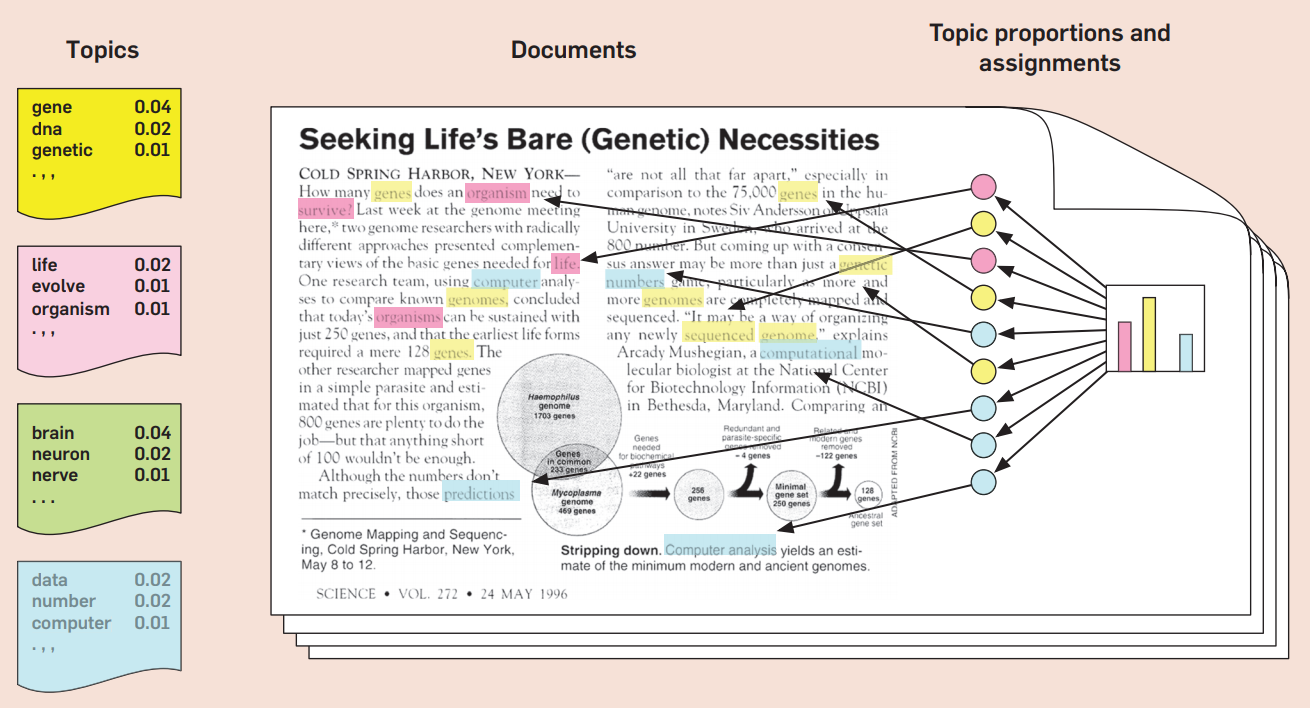
\includegraphics[width=0.8\textwidth]{document/images/lda_topic_model.png}
    % Der Teil in eckigen Klammern ist der Kurztitel für das Table of Contents
    \caption[Schematische Darstellung eines LDA Topic Modelings]{Schematische Darstellung eines LDA Topic Modelings. Quelle: \citetitle{blei_2012} \parencite{blei_2012}}
    \label{fig:lda_example}
\end{figure}

% Wenn wir nicht wollen, dass ein Kapitel auf einer neuen Seite startet, nutzen wir folgenden Befehl hier:
{\let\clearpage\relax \chapter{Theoriefindung}}



%% Bibliography

\setstretch{1.0}
\printbibliography[title={Literaturverzeichnis}]

\end{document}